\documentclass{article}
\usepackage{amsmath}
\usepackage{listings}
\usepackage{xcolor}
\usepackage{graphicx}
\usepackage{geometry}
\usepackage{hyperref}
\usepackage{tikz}
\usetikzlibrary{trees}
\geometry{margin=1in}

\title{Trees}
\author{}
\date{}

\definecolor{codegray}{rgb}{0.5,0.5,0.5}
\definecolor{backcolour}{rgb}{0.95,0.95,0.92}

\lstdefinestyle{cppstyle}{
  backgroundcolor=\color{backcolour},
  commentstyle=\color{codegray},
  keywordstyle=\color{blue},
  numberstyle=\tiny\color{codegray},
  stringstyle=\color{red},
  basicstyle=\ttfamily\footnotesize,
  breakatwhitespace=false,
  breaklines=true,
  captionpos=b,
  keepspaces=true,
  numbers=none,
  numbersep=5pt,
  showspaces=false,
  showstringspaces=false,
  showtabs=false,
  tabsize=2,
  language=C++
}

\begin{document}

\maketitle


A \textbf{tree} is a hierarchical data structure composed of nodes connected by edges. Unlike arrays or linked lists which are \textbf{linear}, trees represent \textbf{non-linear} relationships. This makes them suitable for representing hierarchical models such as file systems, organization charts, and syntax trees.

\section{Tree vs. Linear Structures}
\begin{itemize}
  \item \textbf{Arrays/Linked Lists:} Elements arranged linearly, one after another.
  \item \textbf{Trees:} Each node can have multiple children, forming a hierarchy.
  \item \textbf{Use Cases:} Trees are preferred where branching or hierarchy is essential.
\end{itemize}

\section{Example: Directory Structure}

\begin{figure}[h]
  \centering
  \includegraphics[width=0.6\textwidth]{figs/unix-fs.png}
  \caption{Tree representation of a directory structure}
  \label{fig:dir_tree}
\end{figure}

\section{Terminology}
\begin{itemize}
  \item \textbf{Root:} The topmost node
  \item \textbf{Parent:} A node with child nodes
  \item \textbf{Child:} A node that descends from another node
  \item \textbf{Leaf:} A node with no children
  \item \textbf{Subtree:} A tree formed by a node and its descendants
  \item \textbf{Depth:} Distance from the root to a node
  \item \textbf{Height:} Length of the longest path to a leaf
\end{itemize}


\section{Tree traversal}

\textbf{Preorder Traversal} visits nodes in the order:

\begin{center}
\texttt{Root → Children (Left to Right)}
\end{center}

That is, it first processes the current node, then recursively visits each child subtree. This is useful when you want to copy or serialize the entire structure from the top down.

\textbf{Postorder Traversal} visits nodes in the order:

\begin{center}
\texttt{Children (Left to Right) → Root}
\end{center}

It first traverses all child subtrees recursively, and then processes the current node. This is useful for tasks such as deleting the tree or evaluating expression trees (bottom-up computation).

\textbf{Example Tree:}

\begin{center}
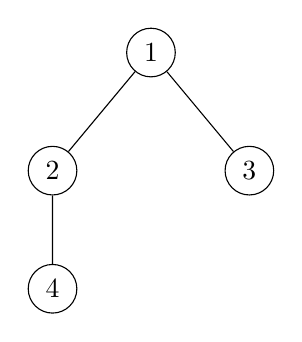
\begin{tikzpicture}[
  level 1/.style={sibling distance=25mm},
  level 2/.style={sibling distance=15mm},
  every node/.style={circle,draw}
]
\node {1}
  child {node {2}
    child {node {4}}
  }
  child {node {3}};
\end{tikzpicture}
\end{center}


\textbf{Preorder:} 1 → 2 → 4 → 3

\textbf{Postorder:} 4 → 2 → 3 → 1

\section{C++ Representation of a Tree}

Below is a basic representation of a general tree where each node can have multiple children.

We define a \texttt{TreeNode} struct for individual nodes and a \texttt{Tree} class that manages the tree and includes traversal methods as member functions.

\begin{lstlisting}[style=cppstyle]
#include <iostream>
#include <vector>
using namespace std;

struct TreeNode {
  int data;
  vector<TreeNode*> children;
  TreeNode(int val) : data(val) {}
};

class Tree {
public:
  TreeNode* root;

  Tree(int rootVal) {
    root = new TreeNode(rootVal);
  }

  // helper to add a new child under 'parent'
  TreeNode* addChild(TreeNode* parent, int val) {
    TreeNode* node = new TreeNode(val);
    parent->children.push_back(node);
    return node;
  }

  // preorder traversal
  void preorder(TreeNode* node) const {
    if (!node) return;
    cout << node->data << " ";
    for (TreeNode* c : node->children)
      preorder(c);
  }
  void preorder() const { preorder(root); }

  // postorder traversal
  void postorder(TreeNode* node) const {
    if (!node) return;
    for (TreeNode* c : node->children)
      postorder(c);
    cout << node->data << " ";
  }
  void postorder() const { postorder(root); }
};
\end{lstlisting}

\textbf{Usage:}
\begin{lstlisting}[style=cppstyle]
Tree t(1);
TreeNode* n2 = t.addChild(t.root, 2);
TreeNode* n3 = t.addChild(t.root, 3);
TreeNode* n4 = t.addChild(n2, 4);

t.preorder();   // prints: 1 2 4 3
t.postorder();  // prints: 4 2 3 1
\end{lstlisting}




\subsection*{Note}
For binary trees (each node has at most 2 children), `inorder` traversal is also common (Left → Root → Right), but is not applicable to general trees.

\section{Practice problem}
Leetcode Problem 104: \textit{Tree height}

\url{https://leetcode.com/problems/maximum-depth-of-binary-tree/description}

\end{document}